
\begin{figure}[h!]
\centering
\caption{Gasto del GNC}
\label{fig:Gasto}
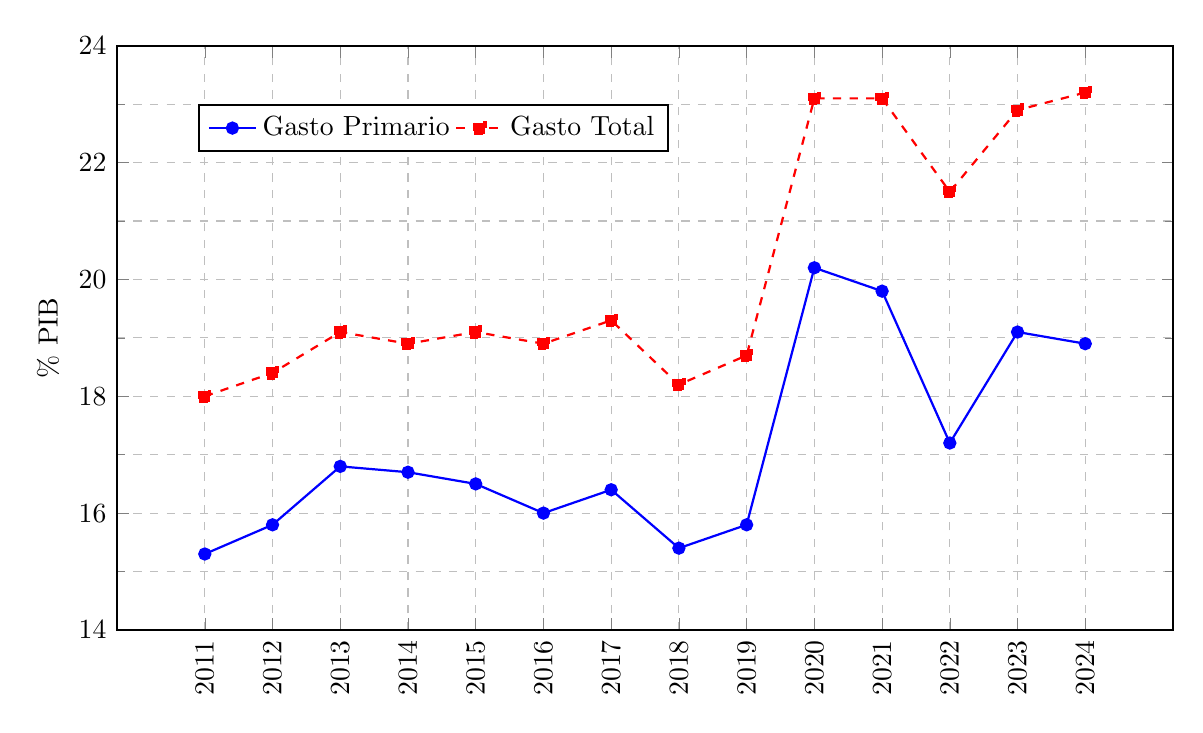
\begin{tikzpicture}
\begin{axis}[
    width=15cm,
    height=9cm,
    %xlabel={Años},
    ylabel={\% PIB},
    xtick=data,
    xticklabels={
    %    {2004}, {2005}, {2006}, {2007}, {2008}, {2009}, {2010}, 
    {2011}, {2012}, {2013},
        {2014}, {2015}, {2016}, {2017}, {2018}, {2019}, {2020}, {2021}, {2022}, {2023}, {2024}
    },
    x tick label style={rotate=90, anchor=east},
    ymin=14,
    ymax=24,
    grid=both,
    grid style=dashed,
    minor y tick num=1,
    legend style={at={(0.3,0.9)}, anchor=north, legend columns=-1},
    thick
]

% Gasto Primario
\addplot[
    color=blue,
    mark=*,
    solid
] coordinates {
    %(0,14.0) (1,14.4) (2,14.4) (3,14.0) (4,14.8) (5,16.5) (6,14.9) 
    (7,15.3) (8,15.8) 
    (9,16.8) (10,16.7) (11,16.5) (12,16.0) (13,16.4) (14,15.4) (15,15.8) (16,20.2) 
    (17,19.8) (18,17.2) (19,19.1) (20,18.9)
};

% Gasto Total
\addplot[
    color=red,
    mark=square*,
    dashed
] coordinates {
    %(0,17.6) (1,17.5) (2,18.1) (3,17.8) (4,18.0) (5,19.5) (6,17.6) 
    (7,18.0) (8,18.4) 
    (9,19.1) (10,18.9) (11,19.1) (12,18.9) (13,19.3) (14,18.2) (15,18.7) (16,23.1) 
    (17,23.1) (18,21.5) (19,22.9) (20,23.2)
};

\legend{Gasto Primario, Gasto Total}
\end{axis}
\end{tikzpicture}
\par \footnotesize{\textit{Fuente: \textcite{minhacienda_balance_2025}}}
\end{figure}
